% ===== UNIT 38: Cost: scalable sparse implementation + figure (6.4 part 3) =====
% Status: REWRITTEN  (change to REWRITTEN / REVIEWED when done; see CHECKLIST.md)
% Rules: style rewrite only. Keep every \cite, \ref, \label, number, equation and table value as is. Change the wording, not the content.
\paragraph{A scalable sparse implementation.} The memory wall comes from the dense implementation, not from the algorithm. We benchmarked a sparse top-$k$ variant. It builds only the first $k_1{+}1$ rank columns and stores $V$ as a sparse matrix ($\mathcal{O}(Nk_1)$ memory). Otherwise it follows the official computation (squared max-normalised distances, $2/3$-rule expansion, LQE). In-domain it matches the dense version to 0.07\,pp (89.92 vs.\ 89.99\% mAP, Rank-1 97.91 vs.\ 97.79). It is also faster (32 vs.\ 44\,s) and uses a 7.9\,MB working set versus 703\,MB for the dense version. At $N{=}41{,}861$ it takes 91\,s versus 254\,s (34.03 vs.\ 34.85\% mAP, both below the 35.9\% AQE-only transfer result). At $N{=}138{,}517$ the dense state alone takes 77\,GB, but the sparse version runs. It takes 372\,s with an 85\,MB sparse $V$, and its AQE-only reference reproduces Table~\ref{tab:veriwild} exactly (23.84\%). This separates the two failure modes. The cost wall can be removed by a better implementation. But re-ranking still reduces transfer accuracy at this scale (22.22 vs.\ 23.84\% mAP). So the domain-specific accuracy failure comes from the geometry of the transferred features, not from the implementation. For in-domain deployment, the sparse variant makes the $+5.5$\,pp re-ranking step practical at gallery scales where the dense version is not. The same idea is used in the re-ranking module of our released tracking pipeline. It finds the top-$k$ neighbourhoods with a FAISS index and stores them per node. It then builds one small local similarity matrix over only the nodes that appear in the candidate pairs and their neighbours, instead of a full $N \times N$ matrix. Figure~\ref{fig:cost}b compares the two.

\begin{figure*}[!t]
  \centering
  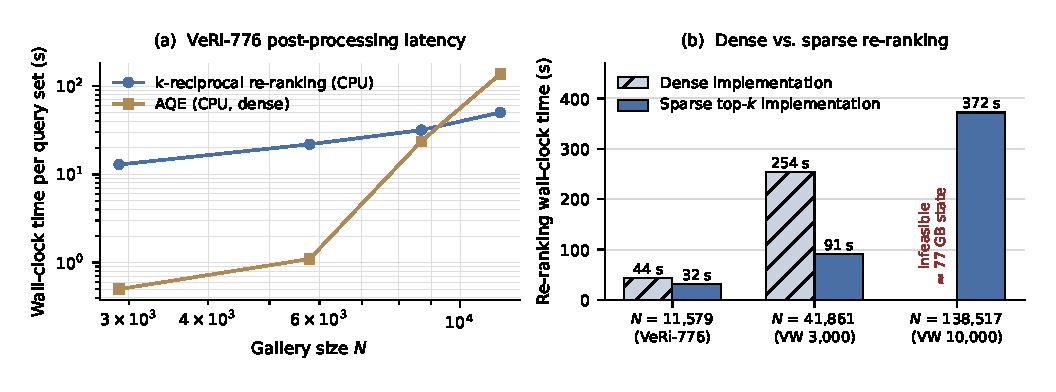
\includegraphics[width=\textwidth]{Fig11}
  \caption{Post-processing cost. \textbf{a} Latency of AQE and $k$-reciprocal
  re-ranking versus gallery size on VeRi-776 (CPU, one query set of 1{,}678
  queries), on logarithmic axes. \textbf{b} Dense versus sparse top-$k$
  re-ranking across three gallery scales. At $N{=}138{,}517$ the dense
  pairwise-distance state alone requires approximately 77\,GB and the
  measurement is infeasible. The sparse implementation completes in
  372\,s at matching accuracy}
  \label{fig:cost}
\end{figure*}
